\section{Work and energy}

	\setcounter{equation}{0}
	\subsection{Work-energy theorem}
		As per Newton's second law, when a particle of mass $m$ moving with a velocity $\vb{v}$ undergoes a force $\vb{F}$ at position $\vb{r}$, we have
		\begin{align*}
			\vb{F}(\vb{r})=m\dv{\vb{v}}{t}
		\end{align*}
		
		\setwrappadding
		\begin{wrapfigure}[6]{r}{0.35\textwidth}
			\centering
			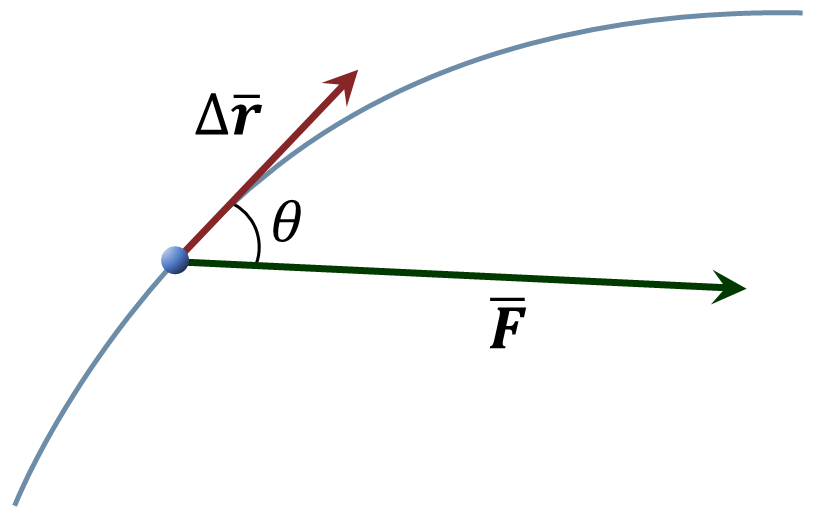
\includegraphics[width=0.32\textwidth]{figures/fig_work-energy-thm-01.png}
		\end{wrapfigure}
		Suppose the particle undergoes a displacement of $\Delta\vb{r}$. Then the work done by the force is
		\resetwrappadding
		\begin{align}
			\Delta W&=\vb{F}\cdot\Delta\vb{r}=m\dv{\vb{v}}{t}\cdot\Delta\vb{r} \label{eqn:delta-W-01}
		\end{align}
		For a time interval $\Delta t$ which is small enough that $\vb{v}$ may be considered to be constant, we can write
		\begin{align*}
			\Delta\vb{r}=\vb{v}\Delta t
		\end{align*}
		Then equation (\ref{eqn:delta-W-01}) becomes
		\begin{align}
			m\dv{\vb{v}}{t}\cdot\Delta\vb{r}&=m\dv{\vb{v}}{t}\cdot\vb{v}\Delta t \label{eqn:delta-W-02}
		\end{align}
		Now, we have
		\begin{align}
			\dv{t}\qty(v^2)&=\dv{t}\qty(\vb{v}\cdot\vb{v}) \nonumber\\
				&=\dv{\vb{v}}{t}\cdot\vb{v}+\vb{v}\cdot\dv{\vb{v}}{t}=2\dv{\vb{v}}{t}\cdot\vb{v} \nonumber\\
			\implies\dv{\vb{v}}{t}\cdot\vb{v}&=\dfrac{1}{2}\dv{t}\qty(v^2) \label{eqn:dvdt-v}
		\end{align}
		
		\setwrappadding
		\begin{wrapfigure}[12]{r}{0.5\textwidth}
			\centering
			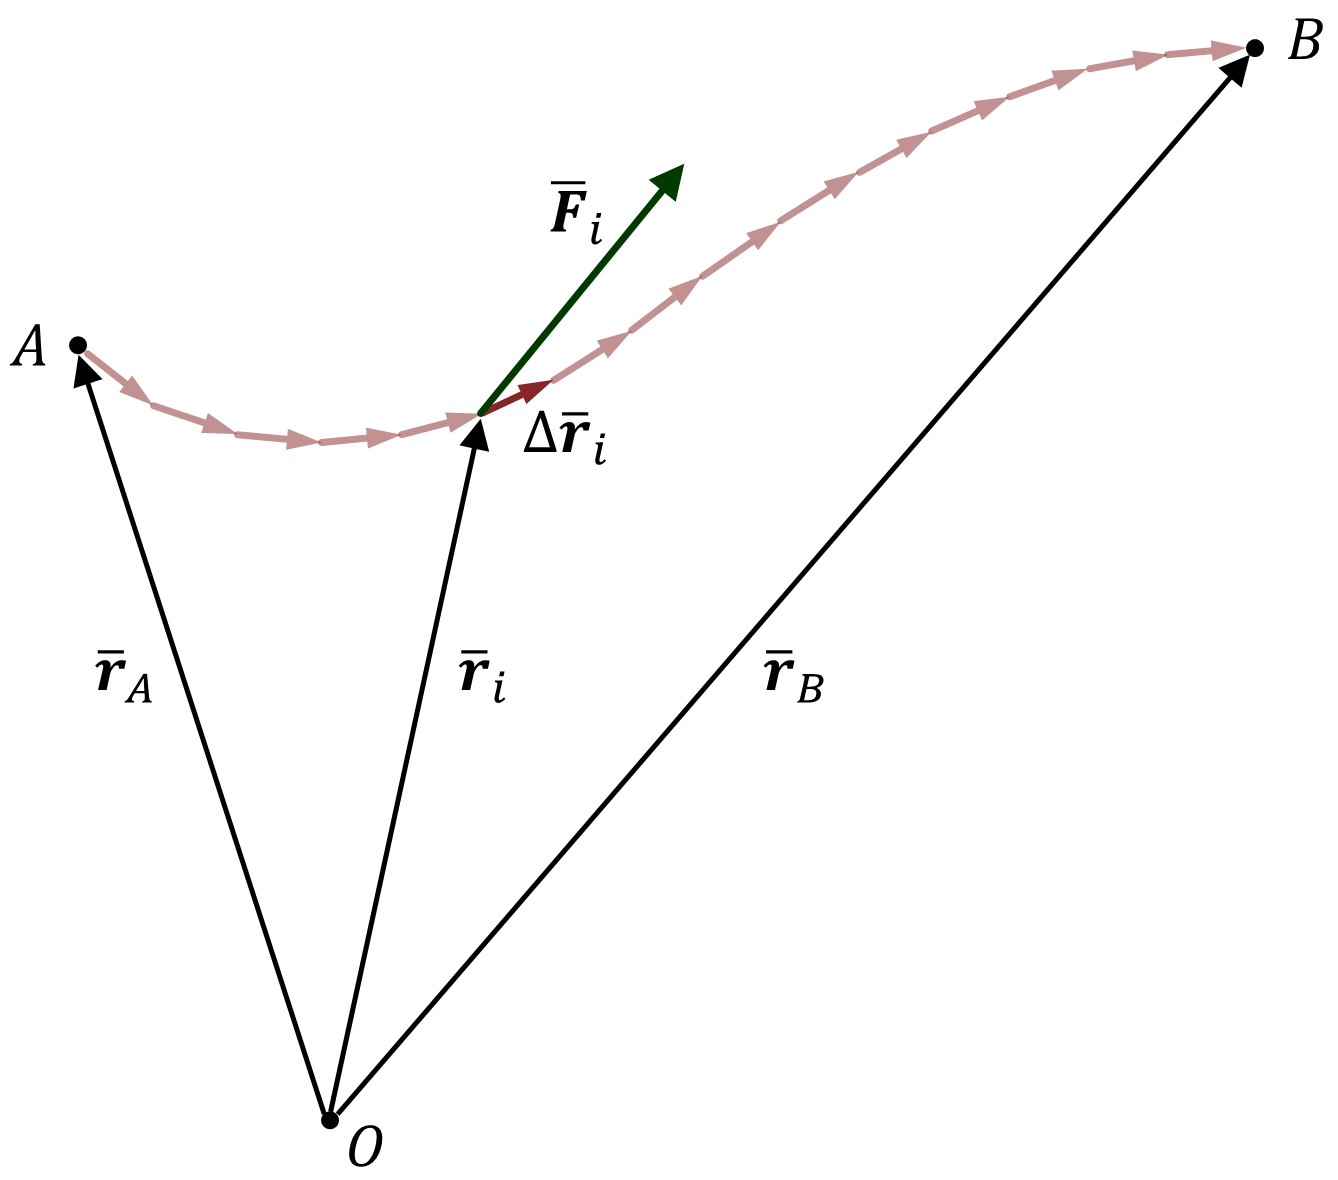
\includegraphics[width=0.48\textwidth]{figures/fig_work-energy-thm-02.png}
		\end{wrapfigure}
		Hence, from equations (\ref{eqn:delta-W-01}), (\ref{eqn:delta-W-02}) and (\ref{eqn:dvdt-v}), we have
		\resetwrappadding		
		\begin{align}
			\vb{F}\cdot\Delta\vb{r}&=\dfrac{1}{2}m\dv{t}\qty(v^2)\Delta t \label{eqn:delta-W-03}
		\end{align}
		
		Suppose now that the path from initial position $A$ to final position $B$ is divided into $N$ small segments. Let $\vb{r}_A$ and $\vb{r}_B$ be the position vectors of the points $A$ and $B$ respectively.
		
		Now, for the $i^\text{th}$ displacement at position $\vb{r}_i$, if the particle undergoes a force $\vb{F}_i$, then the work done over this displacement is obtained from equation (\ref{eqn:delta-W-03}) to be
		\begin{align*}
			\Delta W_i=\vb{F}_i\cdot\Delta\vb{r}_i=\dfrac{1}{2}m\dv{t}\qty(v_i^2)\Delta t_i
		\end{align*}
		Hence the total work done in moving the particle from $A$ to $B$ is obtained by summing over all the $N$ displacements
		\begin{align}
			W&=\sum_{i=1}^{N}{\Delta W_i}=\sum_{i=1}^{N}{\dfrac{1}{2}m\dv{t}\qty(v_i^2)\Delta t_i} \label{eqn:W-sum}
		\end{align}
		
		As the time intervals $\Delta t_i\to 0$, the summation in equation (\ref{eqn:W-sum}) becomes an integral and we have
		\begin{align}
			W&=\int\limits_{t_A}^{t_B}{\dfrac{1}{2}m\dv{t}\qty(v^2)\dd{t}} \nonumber\\
				&=\dfrac{1}{2}m\int\limits_{v_A}^{v_B}{\dd{\qty(v^2)}} \nonumber \\
			\implies W&=\dfrac{1}{2}mv_B^2-\dfrac{1}{2}mv_A^2 \label{eqn:W-T-thm-01}
		\end{align}
		
		In equation (\ref{eqn:W-T-thm-01}), we recognise the terms on the RHS to be the kinetic energies of the particle at positions $B$ and $A$ respectively. Hence we can write
		\begin{align*}
			W&=T_B-T_A
		\end{align*}
		
		The above result may be generalised in the form of the \emph{work-energy theorem}, which states that \emph{the total work done on a system equals the change in its kinetic energy}.
		\begin{align*}
			\boxed{W_\text{total}=\Delta T}
		\end{align*}
	
	\subsection{Potential energy}